\subsection{Penalizing intermediate densities}
\label{subsec:penalization_SIMP}

When dealing with density based topology optimization problems, it is common practice to penalize intermediate values of the design variables.
This is done to encourage the optimization process to find solutions with a more binary distribution of material, which is often more suitable for manufacturing processes.

One of the most common penalization methods is the Solid Isotropic Material with Penalization (SIMP) method.
In particular, the SIMP method is based on the following penalization function:

\begin{equation}
    E(\rho) = E_0 \rho^p
    \label{eq:SIMP_penalization}
\end{equation}

Where $E_0$ is the Young's modulus of the material, $\rho$ is the density of the material at a given point in the domain, and $p$ is the penalization factor.
In order to be effective, the penalization factor $p$ should be chosen such that $p > 1$ and typically $p \approx 3$.

In Figure \ref{fig:SIMP_penalization}, we can see the effect of the penalization factor and how the penalization function behaves for different values of $p$.

\begin{figure}[H]
    \centering
    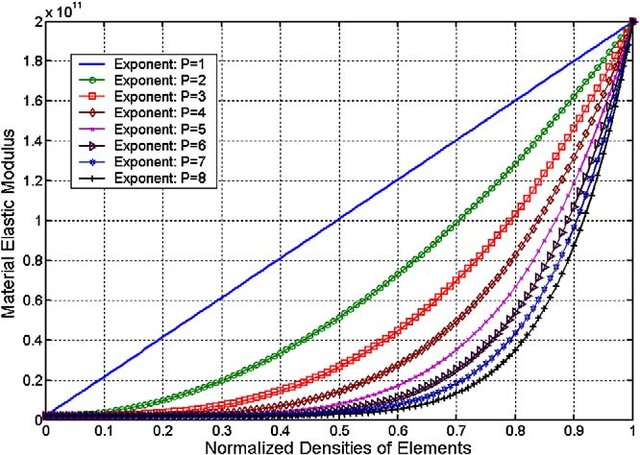
\includegraphics[width=0.6\textwidth]{./img/SIMP_penalizations.jpg}
    \caption{Effect of the penalization factor $p$ on the SIMP penalization function.}
    \label{fig:SIMP_penalization}
\end{figure}

As we can see, for $p = 1$, the penalization function is linear and does not penalize intermediate values of the density.
On the other hand, for $p > 1$, the penalization function becomes more aggressive and penalizes intermediate values more severely.

Of course, by adopting the SIMP method, one should also adjust the optimization algorithm slightly.
In particular, starting from the global stiffness formulation, we observe that:

\begin{equation}
    K(\bm{x}) = \sum_{e=1}^{n} x_e^p K_e^0
    \label{eq:global_stiffness}
\end{equation}

From which we can derive the sensitivity of the compliance function with respect to the design variables:

\begin{equation}
    \frac{\partial C}{\partial x_e} = -\bm{u}^T (p \rho_e^{p-1} K_e^0) \bm{u}
    \label{eq:compliance_sensitivity}
\end{equation}

Because of this new formulation for the sensitivity of the compliance function, we also have to adjust the update rule for the design variables in the optimization algorithm.
In particular, recalling the criteria for the optimality of the design variables in Equation \ref{eq:optimality_criteria}, the previously defined $b_e^k$ term should be updated as follows:

\begin{equation}
    b_e^k = -\frac{\partial C}{\partial y_e} = \bm{u}^T (p \rho_e^{p-1} K_e^0) \bm{u}
    \label{eq:optimality_criteria_SIMP}
\end{equation}

The rest of the optimization algorithm remains unchanged, and the optimization process can proceed as usual.